\chapter{DỮ LIỆU VÀ MÔ HÌNH ĐỀ XUẤT}
\label{ch:mohinh}

Chương này mô tả bộ dữ liệu, quy trình tiền xử lý và kiến trúc mô hình. Mục~\ref{sec:overview} trình bày tổng quan khung mô hình. Các Mục~\ref{sec:data}--\ref{sec:snapshot} mô tả dữ liệu, tập cổ phiếu đủ điều kiện và cách dựng ten-xơ đầu vào. Mục~\ref{sec:graph} trình bày đồ thị tương quan động. Các Mục~\ref{sec:encoder}--\ref{sec:training} trình bày bộ mã hóa thời gian, mạng chú ý đồ thị, tác tử và quy trình huấn luyện. Toàn bộ mô tả trong chương bám sát mã nguồn kèm theo luận văn (Phụ lục~\ref{app:code}).

\section{Tổng quan khung mô hình}
\label{sec:overview}

Hình~\ref{fig:pipeline} minh họa luồng xử lý tại một ngày quyết định $t$. Từ bảng dữ liệu dạng dài (mỗi dòng là một cặp ngày--cổ phiếu), mô hình thực hiện năm bước:
\begin{enumerate}[leftmargin=1.6cm]
  \item \textit{Dựng ảnh chụp thị trường.} Cắt cửa sổ $T=60$ phiên ngay trước $t$ để tạo ten-xơ đặc trưng $X_t\in\R^{N\times T\times F}$ và mặt nạ đủ điều kiện $m_t\in\{0,1\}^N$.
  \item \textit{Mã hóa thời gian.} Bộ mã hóa Transformer biến chuỗi của mỗi cổ phiếu thành một véc-tơ $h_i\in\R^{64}$, trả lời câu hỏi ``mỗi cổ phiếu gần đây trông như thế nào''.
  \item \textit{Xây dựng đồ thị.} Ma trận kề $A_t$ được tính từ tương quan lợi suất trong cùng cửa sổ, trả lời câu hỏi ``cổ phiếu nào liên quan đến cổ phiếu nào''.
  \item \textit{Lan truyền trên đồ thị.} Mạng GAT hai tầng tổng hợp thông tin từ các cổ phiếu lân cận để tạo biểu diễn $z_i\in\R^{64}$ -- trạng thái của tác tử.
  \item \textit{Ra quyết định.} Tác tử PPO chấm điểm từng cổ phiếu, sinh véc-tơ tỷ trọng trên đơn hình; véc-tơ này được chiếu về tập danh mục khả thi (tối đa $K$ mã, mỗi mã không quá $w_{\max}$).
\end{enumerate}
Ba khối có tham số -- bộ mã hóa, mạng đồ thị và tác tử -- được huấn luyện đồng thời bằng một hàm mất mát PPO duy nhất, không có hàm mất mát dự báo phụ trợ.

\begin{figure}[ht]
\centering
\begin{tikzpicture}[font=\footnotesize,
  box/.style={draw, rounded corners=2pt, align=center, minimum height=13mm, minimum width=31mm, inner sep=3pt, fill=white},
  data/.style={box, fill=black!6}, arr/.style={-{Stealth[length=2mm]}, semithick}]
  % hàng trên
  \node[data] (df)   at (0,0)     {Bảng dữ liệu\\(ngày $\times$ cổ phiếu)};
  \node[box]  (snap) at (4.2,0)   {Ảnh chụp tại $t$\\$X_t\in\R^{N\times 60\times 19}$, $m_t$};
  \node[box]  (enc)  at (8.4,0)   {Bộ mã hóa Transformer\\$h_i\in\R^{64}$};
  \node[box]  (gat)  at (12.6,0)  {GAT hai tầng\\$z_i\in\R^{64}$};
  % hàng giữa
  \node[box]  (adj)  at (4.2,-2.6)  {Đồ thị tương quan $A_t$\\$|\rho_{ij}|\ge 0{,}30$};
  \node[box]  (agent) at (12.6,-2.6) {Tác tử PPO\\actor: $\alpha_i\rightarrow$ Dirichlet\\critic: $V(s_t)$};
  % hàng dưới
  \node[box]  (proj) at (8.4,-5.2)  {Chiếu ràng buộc\\top-$K$, trần $w_{\max}$};
  \node[data] (env)  at (4.2,-5.2)  {Môi trường\\lợi suất ròng $r_t$};
  \node[data] (rew)  at (0,-5.2)    {Phần thưởng\\DSR $D_t$};
  \draw[arr] (df) -- (snap); \draw[arr] (snap) -- (enc); \draw[arr] (enc) -- (gat);
  \draw[arr] (df) |- (adj);
  \draw[arr] (adj.east) -- ++(2.6,0) |- ($(gat.west)+(0,-3.5mm)$);
  \draw[arr] (gat) -- (agent);
  \draw[arr] (agent) |- node[pos=0.75, above]{$w_t$} (proj);
  \draw[arr] (proj) -- node[above]{$\tilde w_t$} (env);
  \draw[arr] (env) -- (rew);
  \draw[arr, dashed] (rew.south) -- ++(0,-0.7) -| node[pos=0.25, below]{gradient của hàm mất mát PPO truyền ngược qua tác tử, GAT và bộ mã hóa} ($(agent.south)+(1.1,0)$);
\end{tikzpicture}
\caption{Luồng xử lý của mô hình đề xuất tại một ngày quyết định $t$. Bộ mã hóa thời gian, mạng chú ý đồ thị và tác tử được huấn luyện đầu--cuối bằng hàm mất mát PPO.}
\label{fig:pipeline}
\end{figure}

\section{Dữ liệu}
\label{sec:data}

\subsection{Nguồn dữ liệu}

Dữ liệu bao phủ giai đoạn từ 04/01/2016 đến 31/12/2025 (2.498 phiên giao dịch); dữ liệu năm 2015 được dùng thêm để tính các chỉ báo cần lịch sử cho những phiên đầu năm 2016. Bảng~\ref{tab:sources} tóm tắt các nguồn.

\begin{table}[ht]
\centering\small
\caption{Các nguồn dữ liệu của luận văn}
\label{tab:sources}
\begin{tabularx}{\textwidth}{@{}p{3.6cm}p{2.2cm}X@{}}
\toprule
Nhóm dữ liệu & Tần suất & Nội dung và cách thu thập \\
\midrule
Giá và khối lượng & Ngày & Giá đóng cửa điều chỉnh, khối lượng và giá trị giao dịch của từng mã; thu thập qua API dữ liệu thị trường FireAnt. \\
Báo cáo tài chính & Quý & Bảng cân đối kế toán và báo cáo kết quả kinh doanh của từng doanh nghiệp, kèm \emph{ngày công bố} báo cáo quý; thu thập qua API FireAnt. \\
Hệ số định giá & Ngày & P/E và P/B theo ngày của từng mã \todo{bổ sung tên nguồn}. \\
Vốn hóa thị trường & 6 tháng & Vốn hóa của từng mã tại cuối tháng 6 và cuối tháng 12 hằng năm, dùng để xác định tập cổ phiếu vốn hóa vừa và lớn \todo{bổ sung tên nguồn}. \\
Vĩ mô & Ngày/tháng & Lạm phát (CPI so với cùng kỳ, theo tháng), lợi suất trái phiếu Chính phủ, lãi suất liên ngân hàng qua đêm, tỷ giá USD/VND và lợi suất hằng ngày của VN-Index \todo{bổ sung tên nguồn}. \\
\bottomrule
\end{tabularx}
\end{table}

\subsection{Tập cổ phiếu và điều kiện đủ điều kiện đầu tư}
\label{sec:universe}

Tập cổ phiếu ban đầu gồm các mã từng có vốn hóa trên 5.000 tỷ đồng tại ít nhất một mốc xét trong giai đoạn 2015--2025. Sau khi loại hai chứng chỉ quỹ ETF và chín mã không còn dữ liệu giao dịch (do hủy niêm yết hoặc sáp nhập), tập dữ liệu còn $N=222$ mã, gồm cả cổ phiếu niêm yết trên HOSE, HNX và một số cổ phiếu vốn hóa lớn đăng ký giao dịch trên UPCoM. Việc loại các mã đã hủy niêm yết tạo ra thiên lệch kẻ sống sót (survivorship bias) \cite{brown1992}; hạn chế này được thảo luận ở Mục~\ref{sec:hanche}.

Không phải mã nào cũng được phép đầu tư tại mọi thời điểm. Tại mỗi phiên $s$, cổ phiếu $i$ được gắn nhãn đủ điều kiện $m_i(s)=1$ nếu thỏa mãn đồng thời:
\begin{itemize}
  \item \textit{Điều kiện vốn hóa:} tại mốc xét gần nhất trước hoặc bằng $s$ (cuối tháng 6 hoặc cuối tháng 12), vốn hóa của $i$ lớn hơn 5.000 tỷ đồng. Kết quả của mỗi lần xét có hiệu lực đến mốc xét kế tiếp.
  \item \textit{Điều kiện lịch sử giao dịch:} $i$ đã có lợi suất từ ít nhất 126 phiên trước (khoảng sáu tháng), nhằm bảo đảm đủ dữ liệu cho các chỉ báo và tránh giai đoạn biến động bất thường ngay sau khi lên sàn.
\end{itemize}
Khi dựng ảnh chụp tại ngày quyết định $t$, mặt nạ $m_t$ lấy giá trị nhãn tại phiên cuối của cửa sổ và bổ sung một điều kiện về chất lượng dữ liệu: cổ phiếu bị loại nếu hơn 80\% số phiên trong cửa sổ không có dữ liệu. Cả ba điều kiện chỉ dùng thông tin có trước $t$.

Hình~\ref{fig:eligible} cho thấy số mã đủ điều kiện tăng từ 35 mã (giữa năm 2016) lên 179 mã (năm 2025), phản ánh sự mở rộng của thị trường: trung bình 40 mã trong năm 2016, 89 mã năm 2019, 127 mã năm 2021 và 170 mã năm 2025. Số mã giảm trong năm 2023 (trung bình 131 mã) do vốn hóa của nhiều doanh nghiệp tụt xuống dưới ngưỡng sau đợt suy giảm năm 2022. Vì số nút thay đổi theo thời gian, mọi thành phần của mô hình đều được thiết kế để không phụ thuộc vào $N_t$.

\begin{figure}[ht]
\centering
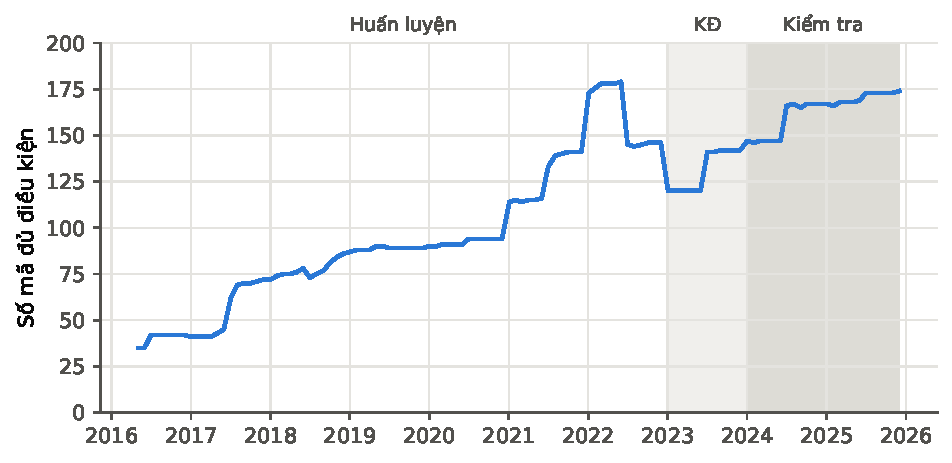
\includegraphics[width=0.88\textwidth]{eligible_universe.pdf}
\caption{Số cổ phiếu đủ điều kiện đầu tư tại mỗi ngày quyết định (tần suất tháng). Hai vùng nền xám lần lượt là giai đoạn kiểm định (2023) và kiểm tra (2024--2025).}
\label{fig:eligible}
\end{figure}

\subsection{Bộ đặc trưng}
\label{sec:features}

Mỗi cổ phiếu tại mỗi phiên được mô tả bằng $F=19$ đặc trưng thuộc ba nhóm (Bảng~\ref{tab:features}).

\begin{table}[ht]
\centering\small
\caption{Bộ 19 đặc trưng đầu vào}
\label{tab:features}
\begin{tabularx}{\textwidth}{@{}p{2.2cm}p{3.3cm}X@{}}
\toprule
Nhóm & Đặc trưng & Định nghĩa \\
\midrule
\multirow{9}{2.2cm}{Giá và kỹ thuật (9)}
 & \texttt{log\_return} & Lợi suất logarit theo ngày, công thức~\eqref{eq:logret} \\
 & \texttt{log\_volume} & Thay đổi logarit của khối lượng: $\ln(V_s/V_{s-1})$ \\
 & \texttt{volatility\_20d/60d} & Độ lệch chuẩn của lợi suất trong 20 và 60 phiên, quy năm ($\times\sqrt{252}$) \\
 & \texttt{rsi\_14} & Chỉ số sức mạnh tương đối 14 phiên \cite{wilder1978} \\
 & \texttt{momentum\_20d/60d} & $\ln(P_s/P_{s-20})$ và $\ln(P_s/P_{s-60})$ \\
 & \texttt{ma\_ratio} & Tỷ số trung bình động 20 phiên trên 50 phiên \\
 & \texttt{log\_amihud\_20d} & Logarit của độ kém thanh khoản Amihud \cite{amihud2002}: trung bình 20 phiên của $|R_s|/\text{GTGD}_s$ \\
\midrule
\multirow{5}{2.2cm}{Tài chính doanh nghiệp (5)}
 & \texttt{PE\_RATIO} & Hệ số giá trên thu nhập \\
 & \texttt{PX\_TO\_BOOK\_RATIO} & Hệ số giá trên giá trị sổ sách \\
 & \texttt{Net income growth} & Tăng trưởng lợi nhuận sau thuế lũy kế bốn quý so với cùng kỳ năm trước \\
 & \texttt{ROE} & Lợi nhuận sau thuế lũy kế bốn quý chia cho vốn chủ sở hữu \\
 & \texttt{A/E} & Đòn bẩy tài chính: tổng tài sản chia cho vốn chủ sở hữu \\
\midrule
\multirow{5}{2.2cm}{Vĩ mô (5)}
 & \texttt{inflation} & Lạm phát CPI so với cùng kỳ \\
 & \texttt{bond\_yield} & Lợi suất trái phiếu Chính phủ \\
 & \texttt{interbank\_rate} & Lãi suất liên ngân hàng qua đêm \\
 & \texttt{vnindex\_return} & Lợi suất hằng ngày của VN-Index \\
 & \texttt{usdvnd\_fx\_rate} & Tỷ giá giữa đồng Việt Nam và đô la Mỹ \\
\bottomrule
\end{tabularx}
\end{table}

\textit{Nhóm giá và kỹ thuật} mô tả xu hướng, rủi ro và thanh khoản gần đây của từng mã. Động lượng 20 và 60 phiên phản ánh hiệu ứng động lượng đã được ghi nhận rộng rãi \cite{jegadeesh1993}; hai thước đo biến động đại diện cho rủi ro riêng; độ kém thanh khoản Amihud đo mức biến động giá trên một đơn vị giá trị giao dịch và đặc biệt có ý nghĩa ở thị trường có thanh khoản phân hóa.

\textit{Nhóm tài chính doanh nghiệp} mô tả định giá, khả năng sinh lời, tăng trưởng và cơ cấu vốn. Các chỉ số tính từ báo cáo tài chính quý chỉ thay đổi khi có báo cáo mới.

\textit{Nhóm vĩ mô} mô tả môi trường chung. Các biến này có cùng giá trị cho mọi cổ phiếu trong một phiên; chúng không giúp phân biệt các mã với nhau tại một thời điểm nhưng cho mô hình biết bối cảnh thị trường.

\subsection{Tránh rò rỉ thông tin tương lai}
\label{sec:leakage}

Rò rỉ thông tin tương lai (look-ahead bias) là sai lầm phổ biến và nghiêm trọng nhất trong kiểm thử ngược. Luận văn áp dụng các nguyên tắc sau:
\begin{itemize}
  \item \textit{Gắn dữ liệu tài chính theo ngày công bố.} Các chỉ số của quý $q$ chỉ được đưa vào dữ liệu từ ngày doanh nghiệp công bố báo cáo quý $q$, không phải từ ngày kết thúc quý; sau đó giá trị được giữ nguyên (điền tiến) đến lần công bố kế tiếp.
  \item \textit{Xét vốn hóa bằng thông tin quá khứ.} Nhãn đủ điều kiện tại phiên $s$ chỉ dùng mốc xét vốn hóa gần nhất không muộn hơn $s$.
  \item \textit{Cửa sổ chỉ gồm các phiên trước ngày quyết định.} Tại ngày quyết định $t$, cả ten-xơ đặc trưng và ma trận tương quan đều được tính từ $T$ phiên có ngày \emph{nhỏ hơn hẳn} $t$.
  \item \textit{Chuẩn hóa trong cửa sổ.} Trung bình và độ lệch chuẩn dùng để chuẩn hóa được tính lại trong từng cửa sổ, không dùng thống kê của toàn bộ mẫu.
  \item \textit{Lợi suất nắm giữ bắt đầu sau ngày quyết định.} Lợi suất của kỳ $t$ được tính trên các phiên thuộc $(t,t^{+}]$, với $t^{+}$ là ngày quyết định kế tiếp (công thức~\eqref{eq:holdret}). Quy ước này tương ứng với việc quan sát dữ liệu đến hết phiên $t-1$, đặt lệnh trong phiên $t$ và được khớp tại giá đóng cửa phiên $t$.
  \item \textit{Chia dữ liệu theo thời gian, không xáo trộn.}
\end{itemize}

\subsection{Chia dữ liệu}

Trục thời gian được chia theo tỷ lệ 70\% -- 10\% -- 20\% số ngày lịch, cho ba giai đoạn liền nhau (Bảng~\ref{tab:split}). Ngày quyết định là phiên giao dịch đầu tiên của mỗi tháng (thiết lập chính) hoặc mỗi tuần (thiết lập bổ sung), tính từ khi đã có đủ 60 phiên lịch sử. Số bước quyết định dùng được ít hơn số ngày quyết định một đơn vị, vì ngày quyết định cuối cùng của mỗi tập không có kỳ nắm giữ tương ứng.

\begin{table}[ht]
\centering\small
\caption{Chia dữ liệu theo thời gian và số ngày quyết định ở hai tần suất tái cân bằng}
\label{tab:split}
\begin{tabular}{@{}lcccc@{}}
\toprule
 & & \multicolumn{2}{c}{Số ngày quyết định} & Số mã đủ điều kiện \\
\cmidrule(lr){3-4}
Tập & Giai đoạn & Tháng & Tuần & (trung bình) \\
\midrule
Huấn luyện & 04/2016 -- 12/2022 & 80 & 349 & 94 \\
Kiểm định & 01/2023 -- 12/2023 & 12 & 52 & 131 \\
Kiểm tra & 01/2024 -- 12/2025 & 24 & 104 & 164 \\
\bottomrule
\end{tabular}
\end{table}

Cần nhấn mạnh quy mô của bài toán dưới góc nhìn học tăng cường: với tái cân bằng theo tháng, toàn bộ ``kinh nghiệm'' của tác tử trong tập huấn luyện chỉ gồm 79 bước quyết định, tập kiểm định có 11 bước và tập kiểm tra có 23 bước. Đây là lượng dữ liệu rất nhỏ so với các bài toán điều khiển mà PPO thường được áp dụng, và là bối cảnh cần ghi nhớ khi diễn giải kết quả ở Chương~\ref{ch:thucnghiem}.

\section{Dựng ten-xơ đầu vào và chuẩn hóa}
\label{sec:snapshot}

Tại ngày quyết định $t$, gọi $s_1<\dots<s_T$ là $T=60$ phiên gần nhất trước $t$. Ten-xơ $X_t\in\R^{N\times T\times F}$ có phần tử $X_t[i,k,f]$ là giá trị đặc trưng $f$ của cổ phiếu $i$ tại phiên $s_k$. Các giá trị thiếu hoặc vô hạn (chẳng hạn thay đổi logarit của khối lượng khi khối lượng bằng không) được thay bằng $0$.

Hai nhóm đặc trưng được chuẩn hóa theo hai cách khác nhau, phù hợp với bản chất của chúng.

\textit{Đặc trưng theo từng mã} (14 đặc trưng thuộc nhóm giá--kỹ thuật và tài chính) được chuẩn hóa \emph{theo lát cắt ngang}: tại mỗi phiên $s_k$,
\begin{equation}
\tilde X_t[i,k,f]=\frac{X_t[i,k,f]-\mu_{k,f}}{\sigma_{k,f}},\qquad
\mu_{k,f}=\frac{1}{N_t}\sum_{j:\,m_{t,j}=1}X_t[j,k,f],
\label{eq:xsec}
\end{equation}
với $\sigma_{k,f}$ là độ lệch chuẩn tương ứng trên các mã đủ điều kiện. Sau phép biến đổi này, giá trị của một đặc trưng cho biết cổ phiếu đang ở vị trí nào \emph{so với các cổ phiếu khác trong cùng phiên} -- chẳng hạn P/E thấp hơn hay cao hơn mặt bằng chung. Cách chuẩn hóa này loại bỏ xu hướng chung của thị trường và sự trôi dạt của thang đo theo thời gian, đồng thời phù hợp với bản chất của bài toán danh mục là so sánh tương đối giữa các mã.

\textit{Đặc trưng vĩ mô} (5 đặc trưng) có cùng giá trị cho mọi mã nên không thể chuẩn hóa theo lát cắt ngang; chúng được chuẩn hóa \emph{theo thời gian} trong cửa sổ:
\begin{equation}
\tilde X_t[i,k,f]=\frac{X_t[i,k,f]-\mu_f}{\sigma_f},
\label{eq:tsnorm}
\end{equation}
với $\mu_f,\sigma_f$ tính trên 60 phiên của cửa sổ. Giá trị sau chuẩn hóa cho biết biến vĩ mô đang cao hay thấp so với chính nó trong ba tháng gần nhất.

Cuối cùng, mọi giá trị được cắt về đoạn $[-10,10]$ để hạn chế ảnh hưởng của ngoại lệ. Khi độ lệch chuẩn nhỏ hơn $10^{-8}$, nó được thay bằng $1$ để tránh chia cho số gần không.

\section{Đồ thị tương quan động}
\label{sec:graph}

\subsection{Xây dựng ma trận kề}

Đồ thị tại ngày quyết định $t$ được xây dựng chỉ từ lợi suất, tách biệt với các đặc trưng khác: mục đích của đồ thị là mô tả sự đồng biến động về giá, không phải sự tương đồng về chỉ số tài chính. Với hai cổ phiếu $i,j$, hệ số tương quan Pearson của lợi suất logarit trong cửa sổ $T_c$ phiên trước $t$ là
\begin{equation}
\rho_{ij}(t)=\corr\big(\ell_{i,s_1:s_{T_c}},\;\ell_{j,s_1:s_{T_c}}\big),
\label{eq:corr}
\end{equation}
được tính trên các phiên mà cả hai mã đều có dữ liệu; nếu số phiên chung nhỏ hơn 30 thì đặt $\rho_{ij}(t)=0$. Ma trận kề có trọng số được định nghĩa bởi
\begin{equation}
A_{ij}(t)=
\begin{cases}
|\rho_{ij}(t)|, & |\rho_{ij}(t)|\ge\tau,\; i\ne j,\\
1, & i=j,\\
0, & \text{còn lại,}
\end{cases}
\label{eq:adj}
\end{equation}
với ngưỡng $\tau=0{,}30$. Giá trị tuyệt đối được dùng vì cả tương quan dương lẫn âm mạnh đều chứa thông tin về quan hệ giữa hai mã; ngưỡng $\tau$ loại các tương quan yếu vốn chủ yếu là nhiễu ước lượng. Sau đó, các cạnh nối tới cổ phiếu không đủ điều kiện bị loại bỏ:
\begin{equation}
\bar A_{ij}(t)=A_{ij}(t)\,m_{t,i}\,m_{t,j},
\label{eq:maskadj}
\end{equation}
nên các nút này bị cô lập hoàn toàn và không tham gia truyền thông điệp.

Trong thiết lập chính, cửa sổ ước lượng trùng với cửa sổ đặc trưng, $T_c=60$ phiên. Để khảo sát quan hệ tương quan \emph{dài hạn} nêu trong tên đề tài, luận văn xét thêm biến thể $T_c=250$ phiên (khoảng một năm giao dịch). Hai lựa chọn thể hiện hai quan niệm khác nhau: cửa sổ ngắn bám sát chế độ thị trường hiện tại nhưng nhiễu hơn; cửa sổ dài cho ước lượng ổn định hơn, phản ánh quan hệ bền vững giữa các doanh nghiệp, nhưng phản ứng chậm khi cấu trúc thị trường thay đổi.

\subsection{Đặc điểm của đồ thị qua các giai đoạn thị trường}

Hình~\ref{fig:density} trình bày mật độ đồ thị -- tỷ lệ cặp cổ phiếu đủ điều kiện có cạnh nối -- theo thời gian cho hai cửa sổ. Có ba quan sát đáng chú ý.

\begin{figure}[ht]
\centering
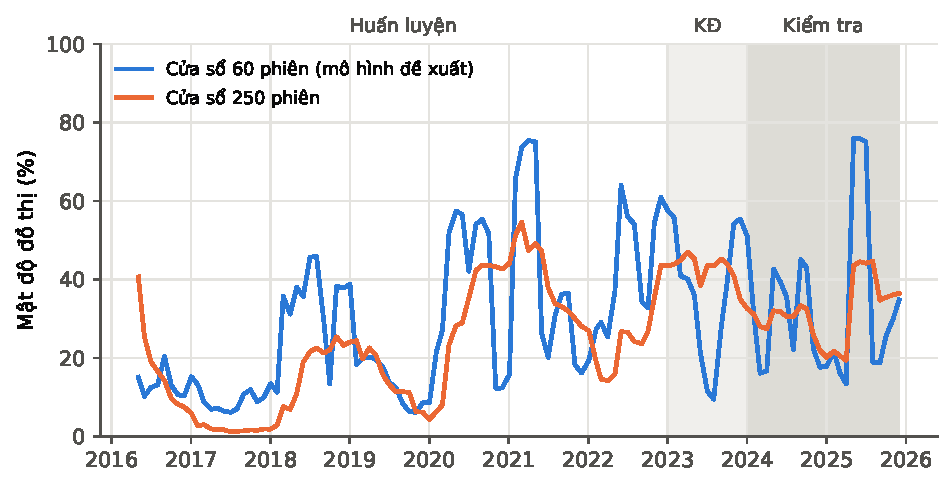
\includegraphics[width=0.9\textwidth]{graph_density.pdf}
\caption{Mật độ của đồ thị tương quan (ngưỡng $\tau=0{,}30$) theo thời gian với cửa sổ ước lượng 60 phiên và 250 phiên.}
\label{fig:density}
\end{figure}

Thứ nhất, cấu trúc đồ thị thay đổi rất mạnh. Với cửa sổ 60 phiên, mật độ trung bình là 30\% nhưng dao động từ 6\% (tháng 11/2019) đến 76\% (tháng 5/2025). Hình~\ref{fig:adjsnap} minh họa hai thái cực này: ở trạng thái thưa, đồ thị chỉ gồm một nhóm nhỏ cổ phiếu liên kết với nhau; ở trạng thái dày, gần như mọi cổ phiếu đều nối với nhau.

Thứ hai, mật độ tăng vọt trong các giai đoạn thị trường căng thẳng: quý I/2020 (COVID-19), các đợt điều chỉnh năm 2021 và 2022, và tháng 4--5/2025. Điều này nhất quán với hiện tượng tương quan tăng khi thị trường giảm mạnh đã được ghi nhận trong tài liệu \cite{longin2001}. Hệ quả đối với mô hình là trong khủng hoảng, đồ thị gần như đầy đủ và ít mang thông tin phân biệt: phép gộp trên lân cận tiến gần tới phép lấy trung bình toàn thị trường.

Thứ ba, đồ thị cửa sổ 250 phiên mượt hơn và phản ứng trễ hơn, đúng như dự đoán. Mật độ của nó duy trì ở mức cao trong khoảng một năm sau mỗi cú sốc, vì các phiên biến động mạnh còn nằm trong cửa sổ ước lượng.

\begin{figure}[ht]
\centering
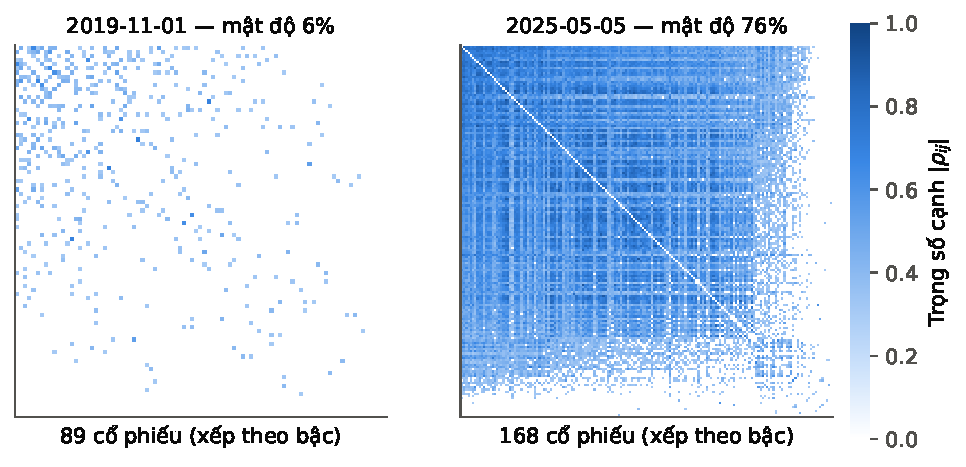
\includegraphics[width=0.95\textwidth]{adjacency_snapshots.pdf}
\caption{Ma trận kề (cửa sổ 60 phiên) tại ngày có mật độ thấp nhất và cao nhất trong giai đoạn 2019--2025. Các cổ phiếu được sắp theo bậc giảm dần; đường chéo được bỏ để dễ quan sát.}
\label{fig:adjsnap}
\end{figure}

Các quan sát này cho thấy giả định đồ thị cố định là không phù hợp với thị trường Việt Nam, và củng cố lý do dùng đồ thị được ước lượng lại theo thời gian. Đồng thời, chúng cũng chỉ ra một hạn chế của việc dùng ngưỡng cố định: số lân cận trung bình của một nút biến thiên từ dưới 3 đến hơn 120, khiến ``tầm nhìn'' của mạng đồ thị rất không đồng đều giữa các thời điểm.

\section{Bộ mã hóa thời gian}
\label{sec:encoder}

Bộ mã hóa ánh xạ chuỗi đặc trưng của mỗi cổ phiếu, $\tilde X_t[i]\in\R^{T\times F}$, thành một véc-tơ $h_i\in\R^{D}$ với $D=64$. Cùng một bộ tham số được dùng cho mọi cổ phiếu; chiều $N$ đóng vai trò chiều lô. Các bước xử lý như sau:
\begin{enumerate}[leftmargin=1.6cm]
  \item \textit{Chiếu đầu vào:} mỗi véc-tơ 19 chiều được chiếu tuyến tính lên không gian 64 chiều.
  \item \textit{Mã hóa vị trí:} cộng mã hóa vị trí dạng sin theo công thức~\eqref{eq:pe}, sau đó áp dụng dropout.
  \item \textit{Hai tầng Transformer:} mỗi tầng theo cấu trúc pre-norm~\eqref{eq:prenorm} với 4 đầu chú ý, mạng truyền thẳng 256 chiều và dropout $0{,}1$; phép chú ý dùng mặt nạ nhân quả nên biểu diễn tại phiên $s_k$ chỉ phụ thuộc vào các phiên $s_1,\dots,s_k$.
  \item \textit{Gộp theo thời gian:} lấy trung bình biểu diễn trên 60 phiên.
  \item \textit{Chiếu đầu ra:} một tầng tuyến tính và chuẩn hóa theo tầng cho $h_i$.
\end{enumerate}
Sau cùng, biểu diễn của các cổ phiếu không đủ điều kiện được đặt bằng không: $h_i\leftarrow m_{t,i}\,h_i$.

Vì toàn bộ cửa sổ đã nằm trước ngày quyết định, mặt nạ nhân quả ở đây không nhằm ngăn rò rỉ thông tin tương lai mà đóng vai trò một thiên kiến quy nạp: nó buộc mô hình xử lý chuỗi theo chiều thời gian. Bộ mã hóa Transformer có 105.536 tham số. Để phục vụ phép loại bỏ thành phần, luận văn cài đặt thêm hai bộ mã hóa hồi quy có cùng giao diện: LSTM hai tầng với 128 đơn vị ẩn (241.088 tham số) và GRU có cấu trúc tương đương (183.232 tham số), trong đó trạng thái ẩn cuối cùng của tầng trên được chiếu về 64 chiều.

\section{Mạng chú ý đồ thị}
\label{sec:gat}

Mạng đồ thị nhận ma trận biểu diễn $H=[h_1,\dots,h_N]\T$ và ma trận kề đã lọc $\bar A_t$, trả về $Z=[z_1,\dots,z_N]\T$. Luận văn tự cài đặt GAT ở dạng ma trận đặc, phù hợp với đồ thị có vài trăm nút và mật độ cao.

\textit{Tầng thứ nhất} dùng $4$ đầu chú ý, mỗi đầu có 16 chiều, tính theo các công thức~\eqref{eq:gat-e}--\eqref{eq:gat-h}; kết quả của các đầu được ghép nối thành véc-tơ 64 chiều và đưa qua hàm kích hoạt ELU:
\begin{equation}
h_i^{(1)}=\ELU\Big(\big\Vert_{k=1}^{4}\sum_{j\in\mathcal{N}(i)}\alpha_{ij}^{(k)}W^{(k)}h_j\Big).
\end{equation}
\textit{Tầng thứ hai} dùng một đầu chú ý với 64 chiều đầu ra, theo sau là chuẩn hóa theo tầng:
\begin{equation}
z_i=\LN\Big(\sum_{j\in\mathcal{N}(i)}\alpha_{ij}'\,W'h_j^{(1)}\Big).
\end{equation}
Hệ số dốc của LeakyReLU là $0{,}2$ và dropout $0{,}1$ được áp dụng lên các hệ số chú ý. Với hai tầng, biểu diễn của mỗi cổ phiếu tích hợp thông tin từ các cổ phiếu cách nó tối đa hai bước trên đồ thị. Biểu diễn của các nút không đủ điều kiện được đặt bằng không ở đầu ra.

Như đã lưu ý ở Chương~\ref{ch:lythuyet}, trong cài đặt này ma trận kề chỉ xác định tập lân cận $\mathcal{N}(i)=\{j:\bar A_{ij}\ne0\}$; độ lớn $|\rho_{ij}|$ không tham gia trực tiếp vào hệ số chú ý. Mạng GAT có 8.576 tham số.

\textit{Biến thể đối chứng.} Để đánh giá vai trò của cơ chế chú ý và của bản thân đồ thị, luận văn dùng hai biến thể: (i) GCN hai tầng theo công thức~\eqref{eq:gcn}, trong đó trọng số gộp được xác định cố định bởi $\bar A_t$ đã chuẩn hóa đối xứng (8.448 tham số) -- biến thể này \emph{có} dùng độ lớn của tương quan; và (ii) biến thể ``không đồ thị'', giữ nguyên kiến trúc GAT nhưng thay $\bar A_t$ bằng ma trận chỉ có khuyên, nên mỗi cổ phiếu không nhận thông tin từ cổ phiếu khác.

\section{Tác tử và không gian hành động}
\label{sec:agent}

\subsection{Trạng thái, hành động và chính sách}

\textit{Trạng thái} tại bước $t$ là ma trận biểu diễn $Z_t\in\R^{N\times D}$ cùng mặt nạ $m_t$. \textit{Hành động} là véc-tơ tỷ trọng $w_t$ trên các mã đủ điều kiện.

\textit{Actor} là một mạng hai tầng (64 đơn vị ẩn, kích hoạt ReLU) áp dụng riêng rẽ cho từng cổ phiếu với tham số dùng chung, cho một điểm số vô hướng $u_i$; điểm số được biến đổi thành tham số tập trung dương
\begin{equation}
\alpha_i=\softplus(u_i)+10^{-3}.
\label{eq:alpha}
\end{equation}
Chính sách là phân phối Dirichlet trên các mã đủ điều kiện (Mục~\ref{sec:dirichlet}):
\begin{equation}
w_t\big|_{\{i:\,m_{t,i}=1\}}\sim\Dir\big(\alpha_i:\,m_{t,i}=1\big),\qquad w_{t,i}=0\ \text{nếu}\ m_{t,i}=0 .
\label{eq:policy}
\end{equation}
Khi huấn luyện, $w_t$ được lấy mẫu từ phân phối này để khám phá; khi đánh giá, hành động tất định là kỳ vọng $w_{t,i}=\alpha_i/\sum_j\alpha_j$ theo~\eqref{eq:dir-mean}. Vì actor chấm điểm từng mã bằng cùng một mạng, chính sách không phụ thuộc vào số lượng hay thứ tự của các cổ phiếu, phù hợp với tập cổ phiếu thay đổi theo thời gian.

\textit{Critic} ước lượng giá trị của trạng thái từ biểu diễn trung bình của các mã đủ điều kiện:
\begin{equation}
V_\phi(s_t)=g_\phi\Big(\frac{1}{N_t}\sum_{i:\,m_{t,i}=1}z_i\Big),
\end{equation}
với $g_\phi$ là mạng hai tầng có 64 đơn vị ẩn. Actor và critic có tổng cộng 8.450 tham số; toàn bộ mô hình có khoảng 122,6 nghìn tham số.

\subsection{Chiếu về tập danh mục khả thi}
\label{sec:projection}

Một mẫu Dirichlet phân bổ tỷ trọng dương cho mọi mã đủ điều kiện, trong khi danh mục thực tế bị giới hạn về số mã và mức tập trung. Do đó $w_t$ được chiếu về tập khả thi bằng một phép biến đổi tất định $\Pi_{K,w_{\max}}$:
\begin{enumerate}[leftmargin=1.6cm]
  \item giữ lại $K=20$ mã có tỷ trọng lớn nhất, đặt các mã còn lại bằng không, rồi chuẩn hóa để tổng bằng 1;
  \item nếu có mã vượt trần $w_{\max}=10\%$, cắt mã đó về $w_{\max}$ và phân phối phần dư cho các mã chưa chạm trần theo tỷ lệ tỷ trọng hiện có; lặp lại đến khi không còn mã nào vượt trần.
\end{enumerate}
Với $K=20$ và $w_{\max}=10\%$, mỗi mã được nắm giữ có tỷ trọng trung bình 5\% và không quá 10\%.

Về mặt hình thức, phép chiếu được coi là \emph{một phần của môi trường}: hành động của tác tử vẫn là mẫu Dirichlet $w_t$ (dùng để tính xác suất trong hàm mục tiêu PPO), còn môi trường thực thi danh mục $\tilde w_t=\Pi_{K,w_{\max}}(w_t)$ và trả về phần thưởng tương ứng. Cách xử lý này hợp lệ đối với thuật toán gradient chính sách, nhưng nó tạo ra một ánh xạ nhiều--một từ hành động sang danh mục thực thi; ảnh hưởng của điều này đến việc học được phân tích ở Mục~\ref{sec:policy-behaviour}.

\subsection{Phần thưởng}

Lợi suất ròng của bước $t$ được tính theo~\eqref{eq:netret} với danh mục thực thi:
\begin{equation}
r_t=\tilde w_t\T R_t-c\,\lVert\tilde w_t-\tilde w_{t-1}\rVert_1,\qquad c=10\ \text{điểm cơ bản},
\end{equation}
trong đó $R_t$ là véc-tơ lợi suất nắm giữ trong kỳ; cổ phiếu không có dữ liệu giá trong kỳ được gán lợi suất bằng không. Phần thưởng là tỷ số Sharpe vi phân~\eqref{eq:dsr} của chuỗi $r_t$ với $\eta=0{,}01$. Ở bước đầu tiên của mỗi quỹ đạo, các mô-men được khởi tạo $A_1=r_1$, $B_1=r_1^2$ và phần thưởng bằng không; khi phương sai trượt nhỏ hơn ngưỡng số học, phần thưởng cũng được đặt bằng không. Cuối cùng, phần thưởng được cắt về đoạn $[-5,5]$:
\begin{equation}
\text{phần thưởng}_t=\clip(D_t,-5,5).
\label{eq:reward}
\end{equation}

\section{Quy trình huấn luyện đầu--cuối}
\label{sec:training}

Thuật toán~\ref{alg:train} tóm tắt quy trình huấn luyện. Mỗi vòng lặp gồm hai pha.

\textit{Pha thu thập (rollout).} Tác tử chạy tuần tự qua toàn bộ các ngày quyết định của tập huấn luyện theo thứ tự thời gian, tạo thành \emph{một} quỹ đạo. Tại mỗi bước, mô hình tính $Z_t$, lấy mẫu hành động, môi trường trả về lợi suất ròng và phần thưởng. Pha này không tính gradient; hành động, logarit xác suất và giá trị ước lượng được lưu lại.

\textit{Pha cập nhật.} Lợi thế được tính bằng GAE~\eqref{eq:gae} với $\gamma=0{,}99$, $\lambda=0{,}95$ rồi chuẩn hóa về trung bình không và phương sai đơn vị. Trong mỗi epoch, phép tính xuôi qua bộ mã hóa và mạng đồ thị được \emph{thực hiện lại} cho từng bước để gradient của hàm mất mát~\eqref{eq:ppo-loss} truyền ngược qua cả ba khối; gradient được cộng dồn trên toàn bộ quỹ đạo, cắt chuẩn về 1 rồi cập nhật một lần bằng Adam \cite{kingma2015}. Như vậy mỗi vòng lặp gồm $E_{\mathrm{ppo}}=4$ bước gradient trên toàn lô.

\textit{Chọn mô hình.} Sau mỗi vòng lặp, chính sách tất định được chạy trên tập kiểm định và tỷ số Sharpe quy năm được ghi lại; bộ tham số có tỷ số Sharpe kiểm định cao nhất được giữ làm mô hình cuối cùng.

\begin{algorithm}[ht]
\caption{Huấn luyện đầu--cuối mô hình Transformer--GAT--PPO}
\label{alg:train}
\small
\begin{algorithmic}[1]
\Require Dữ liệu huấn luyện và kiểm định; phí $c$; ngưỡng cắt $\epsilon$; số vòng lặp $N_{\mathrm{iter}}$; số epoch $E_{\mathrm{ppo}}$
\Ensure Tham số $\theta^{*}$ của bộ mã hóa $f_{\mathrm{enc}}$, mạng đồ thị $f_{\mathrm{gat}}$ và tác tử $(\pi,V)$
\State Dựng trước $(X_t,m_t,\bar A_t,R_t)$ cho mọi ngày quyết định $t$
\For{vòng lặp $=1,\dots,N_{\mathrm{iter}}$}
  \State Khởi tạo lại bộ ước lượng DSR; $\tilde w_{0}\gets 0$
  \For{mỗi ngày quyết định $t$ của tập huấn luyện} \Comment{pha thu thập, không gradient}
    \State $Z_t\gets f_{\mathrm{gat}}\big(m_t\odot f_{\mathrm{enc}}(X_t),\bar A_t\big)$
    \State Lấy mẫu $w_t\sim\Dir(\alpha(Z_t))$; lưu $\log\pi(w_t\mid Z_t)$ và $V(Z_t)$
    \State $\tilde w_t\gets\Pi_{K,w_{\max}}(w_t)$;\quad $r_t\gets\tilde w_t\T R_t-c\lVert\tilde w_t-\tilde w_{t-1}\rVert_1$
    \State Phần thưởng $\gets\clip(D_t,-5,5)$ với $D_t$ theo~\eqref{eq:dsr}
  \EndFor
  \State Tính lợi thế $\hat A_t$ bằng GAE và mục tiêu $\hat G_t$; chuẩn hóa $\hat A_t$
  \For{epoch $=1,\dots,E_{\mathrm{ppo}}$} \Comment{pha cập nhật}
    \State Tính lại $Z_t$ có gradient cho mọi $t$; cộng dồn gradient của hàm mất mát~\eqref{eq:ppo-loss}
    \State Cắt chuẩn gradient về 1; cập nhật $\theta$ bằng Adam
  \EndFor
  \State Tính tỷ số Sharpe của chính sách tất định trên tập kiểm định; lưu $\theta$ nếu tốt nhất
\EndFor
\State \Return bộ tham số có tỷ số Sharpe kiểm định cao nhất
\end{algorithmic}
\end{algorithm}

Bảng~\ref{tab:hyper} liệt kê các siêu tham số. Chúng được giữ cố định cho mọi thực nghiệm; luận văn không tinh chỉnh siêu tham số trên tập kiểm tra.

\begin{table}[ht]
\centering\small
\caption{Cấu hình mô hình và siêu tham số huấn luyện}
\label{tab:hyper}
\begin{tabular}{@{}llp{6.4cm}@{}}
\toprule
Thành phần & Tham số & Giá trị \\
\midrule
Dữ liệu & Cửa sổ đặc trưng $T$; số đặc trưng $F$ & 60 phiên; 19 \\
 & Ràng buộc danh mục & $K=20$ mã, $w_{\max}=10\%$ \\
 & Phí giao dịch $c$ & 10 điểm cơ bản trên giá trị luân chuyển \\
Đồ thị & Thước đo; cửa sổ; ngưỡng & $|\rho|$ Pearson; 60 phiên (biến thể: 250); $\tau=0{,}30$ \\
 & Số quan sát chung tối thiểu & 30 phiên \\
Bộ mã hóa & Kiến trúc & Transformer pre-norm, 2 tầng, 4 đầu, $d=64$, FFN 256 \\
 & Gộp; dropout & trung bình theo thời gian; $0{,}1$ \\
GAT & Tầng 1 / tầng 2 & 4 đầu $\times$ 16 chiều (ghép), ELU / 1 đầu $\times$ 64 chiều \\
Tác tử & Actor / critic & MLP 64--64--1 (theo từng mã) / MLP 64--64--1 (sau gộp trung bình) \\
 & Chính sách & Dirichlet, $\alpha_i=\softplus(u_i)+10^{-3}$ \\
PPO & $\epsilon$; epoch mỗi vòng; $\gamma$; $\lambda$ & $0{,}2$; 4; $0{,}99$; $0{,}95$ \\
 & $c_v$; $c_e$; cắt gradient & $0{,}5$; $0{,}01$; chuẩn $\le 1$ \\
 & Bộ tối ưu; tốc độ học & Adam; $3\times10^{-4}$ \\
Phần thưởng & DSR: $\eta$; biên độ cắt & $0{,}01$; $\pm5$ \\
Chọn mô hình & Tiêu chí & Tỷ số Sharpe cao nhất trên tập kiểm định \\
\bottomrule
\end{tabular}
\end{table}

\section{Tổng kết chương}

Chương này đã mô tả bộ dữ liệu 222 mã cổ phiếu Việt Nam giai đoạn 2016--2025 với 19 đặc trưng thuộc ba nhóm, cùng các nguyên tắc xử lý nhằm tránh rò rỉ thông tin tương lai. Tập cổ phiếu đủ điều kiện thay đổi theo thời gian, từ 35 đến 179 mã. Đồ thị tương quan được ước lượng lại tại mỗi ngày quyết định; khảo sát cho thấy mật độ của nó biến thiên từ 6\% đến 76\% và tăng vọt trong các giai đoạn thị trường căng thẳng. Mô hình đề xuất ghép ba khối -- bộ mã hóa Transformer, mạng GAT hai tầng và tác tử PPO với chính sách Dirichlet -- thành một hệ thống khoảng 122,6 nghìn tham số, huấn luyện đầu--cuối với phần thưởng là tỷ số Sharpe vi phân sau phí giao dịch. Chương tiếp theo trình bày thực nghiệm và kết quả.
